An artificial neuron's activation function defines that neuron's output value
for given inputs, commonly being ${f: \mathbb{R} \rightarrow \mathbb{R}}$ \cite{leskovec2020mining}. A significant trait of many activation functions is their differentiability, allowing them to be used for Backpropagation, ANN algorithm for training weights. Having derivative not saturating or exploding, heads towards 0 or inf, is necessary for activation functions.

For such reasons, the usage of step function or any linear function is unsuitable for ANN.
% Sigmoid Function ==========================================================================================================
\setsecnumdepth{all}
\subsubsection{Sigmoid Function}
The sigmoid function is commonly used in ANN as an alternative to the step function. A popular choice of the sigmoid function is a logistic sigmoid. Its output value is in the range of 0 and 1.

\begin{equation}
    {\sigma(\alpha) = \frac{1}{1 + e^{-\alpha}} = \frac{e^x}{1 + e^{x}}}
\end{equation}


% \begin{figure}[h]
% 	\centering
%     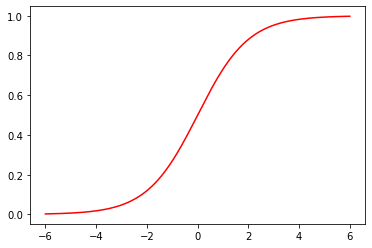
\includegraphics[width=7cm]{sigmoid}
% 	\caption{Sigmoid function}
% 	\label{fig:sigmoid}
% \end{figure}


One of the reasons being the simplicity of derivative calculation:

\begin{equation}
    {\frac{d}{dx}\sigma(\alpha) = \frac{e^x}{(1 + e^{x})^2} = \sigma(x)(1-\sigma(x))}
\end{equation}


One of its disadvantages being the vanishing gradient. A problem where for a given very high or very low input values, there would be almost no change in its prediction. Possibly resulting in training complications or performance issues.\cite{7typesactivationfunctions}

% Hyperbolic Tangent ==========================================================================================================

\subsubsection{Hyperbolic Tangent}

Hyperbolic tangent is similar to logistic sigmoid function with a key difference in its output, ranging between -1 and 1.

\begin{equation}
    {tanh(x) = \frac{e^x - e^{-x}}{e^x + e^{-x}}}
\end{equation}


\begin{figure}[h]
	\centering
    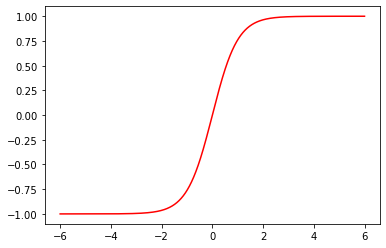
\includegraphics[width=8cm]{tangent}
	\caption{Hyperbolic tangent}
	\label{fig:hyperbolictangent}
\end{figure}


It shares sigmoid's simple calculation of its derivative.

\begin{equation}
    {\frac{d}{dx}tanh(x) = 1 - \frac{(e^x - e^{-x})^2}{(e^x + e^{-x})^2} = 1 -tanh^2(x)}
\end{equation}

By being only moved and scaled version of the sigmoid function, hyperbolic tangent does share sigmoid's advantages and its disadvantages.\cite{leskovec2020mining}

% Rectified Linear Unit ==========================================================================================================

\subsubsection{Rectified Linear Unit}

The output of the rectified linear unit (ReLU) is defined as:

\begin{equation}
    f(x) = max(0,x)
\begin{cases}
    x, & \text{if $x\ \geq\ 0$}\\
    0, & \text{if $x\ <\ 0$}
\end{cases} 
\end{equation} 

\begin{figure}[h]
	\centering
    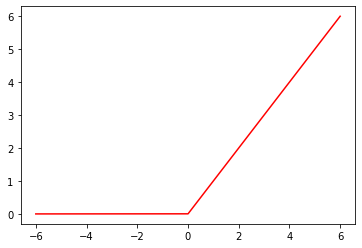
\includegraphics[width=7cm]{relu}
	\caption{Rectified Linear Unit}
	\label{fig:relu}
\end{figure}


ReLU popularity is mainly for its computational efficiency.\cite{7typesactivationfunctions} ReLu's disadvantages appear when inputs approach zero or are negative. Causing the so-called dying ReLu problem, where the network is unable to learn. There are many variations of ReLu to this date, e.g., Leaky ReLU, Parametric ReLU, ELU, ... 
% Softmax ==========================================================================================================

\subsubsection{Softmax}

Softmax separates itself from all the previously mentioned functions by its ability to handle multiple input values in the form of a vector $\vec{x} = (x_1,x_2,...,x_n)$ and output for each $x_i$ defined as:

\begin{equation}
    {\sigma(x_i) = \frac{e^x_i}{\sum_{j=1}^{n}e^x_j}}
\end{equation}


For output being normalized probability distribution, ensuring $\sum_{i}\sigma(x_i) = 1$.\cite{lipton2015critical} It is being used as the last activation function of ANN to normalize the network's output into $n$ probability groups.
